% !TEX root = ../main.tex
% --+ 11.41 SUMMARY +-----------------------------------------------------------
\begin{frame}{FMT Efficiency}
    \label{11.41::summary}
    \begin{itemize}
        \item
            Initially, my plan was to work with run \ef{12933} (10.4 GeV beam, 250 nA), but analysis shows a very poor FMT efficiency.

        \item
            This issue comes from three sources: \ef{alignment}, \ef{reconstruction}, and \ef{geometry}.
    \end{itemize}

    \vspace{-12pt}
    \begin{columns}[onlytextwidth,T]

    \begin{column}{.05\linewidth}\end{column} % Centering column.

    \begin{column}{.49\linewidth}
        \begin{center}
            \begin{figure}[t]
                \centering{
                    \fbox{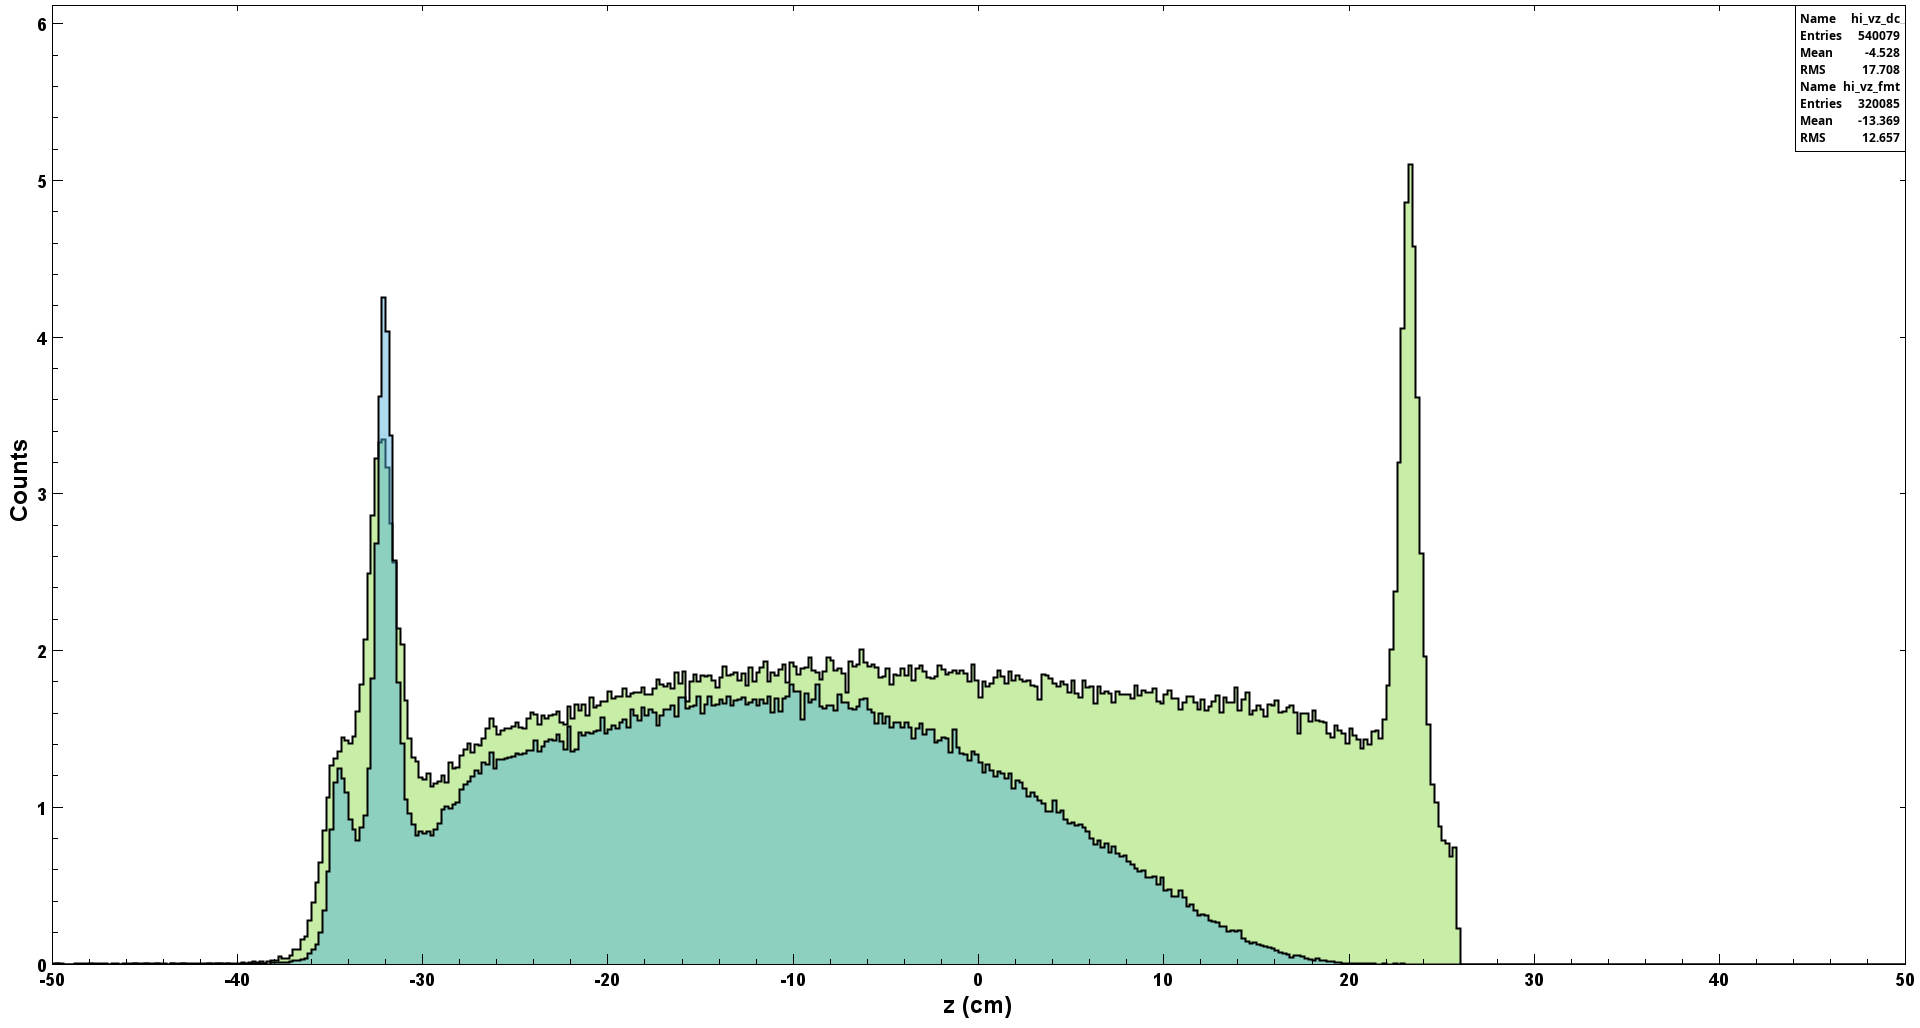
\includegraphics[width=\textwidth]{41vz_011983.png}}
                }
                \textit{Run \ef{11983}, reconstructed in 2020.}
            \end{figure}
        \end{center}
    \end{column}

    \begin{column}{.29\linewidth}
        \begin{center}
            \begin{figure}[t]
                \centering{
                    \fbox{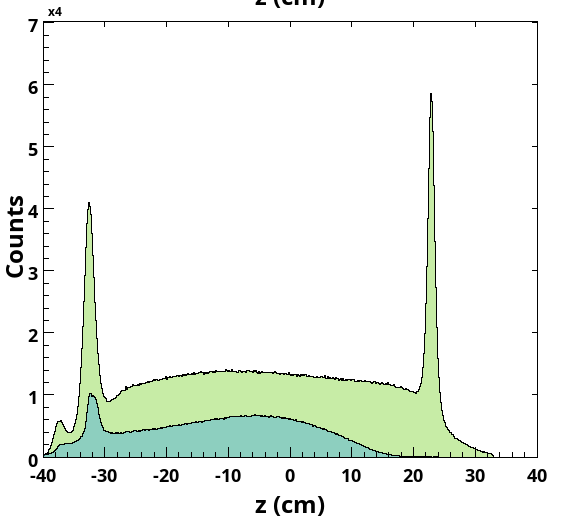
\includegraphics[width=\textwidth]{41vz_012933.png}}
                }
                \textit{Run \ef{12993}, 2023.}
            \end{figure}
        \end{center}
    \end{column}

    \begin{column}{.05\linewidth}\end{column} % Centering column.

    \end{columns}
    \begin{center}
        \textit{\ef{$v_z$} for \textbf{\textcolor[HTML]{c7eca6}{DC (green)}} and \textbf{\textcolor[HTML]{8dcfbf}{FMT (cyan)}} tracks.}
    \end{center}
\end{frame}

% --+ 11.42 ALIGNMENT EFFECT +--------------------------------------------------
\begin{frame}{FMT Efficiency: Alignment Effect}
    \label{11.42::alignment_effect}
    \begin{itemize}
        \item
            Alignment problem comes from an issue with the \ef{Summer 2020} alignment table in the Calibration Constants Database\appref{20.01::ccdb}.

        \item
            To work around this, we switch to \ef{Spring 2020} data.
    \end{itemize}

    \vspace{-12pt}
    \begin{columns}[onlytextwidth,T]

    \begin{column}{.05\linewidth}\end{column} % Centering column.

    \begin{column}{.35\linewidth}
        \begin{center}
            \begin{figure}[t]
                \centering{
                    \fbox{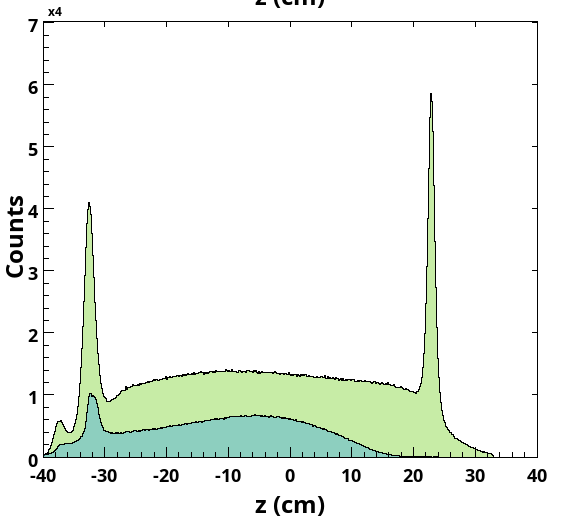
\includegraphics[width=\textwidth]{41vz_012933.png}}
                }
                \textit{Summer run \ef{12933}.}
            \end{figure}
        \end{center}
    \end{column}

    \begin{column}{.35\linewidth}
        \begin{center}
            \begin{figure}[t]
                \centering{
                    \fbox{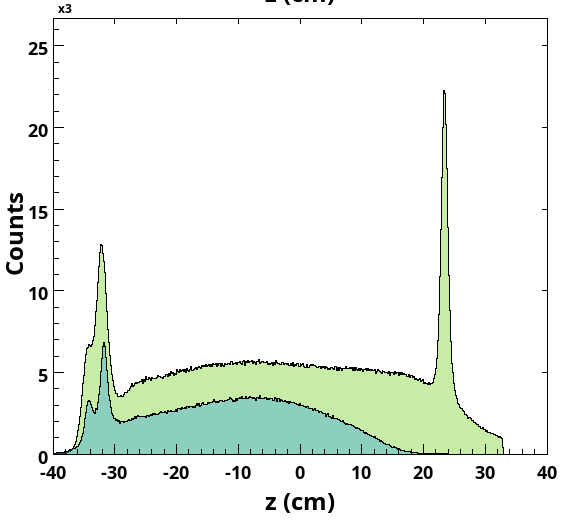
\includegraphics[width=\textwidth]{42vz_012016.png}}
                }
                \textit{Spring run \ef{12016}.}
            \end{figure}
        \end{center}
    \end{column}

    \begin{column}{.05\linewidth}\end{column} % Centering column.

    \end{columns}
    \begin{center}
        \textit{\ef{$v_z$} for \textbf{\textcolor[HTML]{c7eca6}{DC (green)}} and \textbf{\textcolor[HTML]{8dcfbf}{FMT (cyan)}} tracks.}
    \end{center}
\end{frame}

% --+ 11.43 GEOMETRY EFFECT +---------------------------------------------------
\begin{frame}{FMT Efficiency: Geometry Effect}
    \label{11.43::geometry_effect}
    \begin{itemize}
        \item
            Due to its position, FMT has a non-trivial efficiency curve along the \ef{$z$ axis} and \ef{$\theta$ angle}.

        \vspace{6pt}
        \item
            If we want to understand the behavior of DIS variables, we need to study this effect and disentangle it from acceptance.
    \end{itemize}

    \vspace{12pt}
    We can define this \ef{efficiency region} by projecting straight lines between the $z$ axis and the detector\appref{20.02::fmt_acceptance_curve}, such that
    \begin{empheq}[box={\eqbox[5pt][5pt]}]{equation*}
        \theta_\text{min}(z) = 57.29^\circ \cdot \text{atan}\left( \frac{R_\text{min}}{z_0 - z} \right),
        \hspace{10pt}
        \theta_\text{max}(z) = 57.29^\circ \cdot \text{atan}\left( \frac{R_\text{max}}{z_0 - z} \right),
    \end{empheq}
    where \ef{$R_\text{min}$} and \ef{$R_\text{max}$} are the radii of FMT, and \ef{$z_0$} is the first layer's $z$ position.

    \vspace{6pt}
    We then apply a cut on DC and FMT tracks based on this region.
\end{frame}

% --+ 11.44 RECONSTRUCTION EFFECT +---------------------------------------------
\begin{frame}{FMT Efficiency: Reconstruction Effect}
    \label{11.44::reconstruction_effect}
    \begin{itemize}
        \item
            After correcting both effects, FMT efficiency remains low.

        \item
            It was determined that this effect is not correlated with run number, beam energy, or beam luminosity.
            Thus, it is attributed to reconstruction.

        \item
            If we define FMT efficiency as the \ef{\% of DC tracks that get accepted by FMT}\appref{20.03::fmt_efficiency_error_estimation}, we see:
    \end{itemize}

    \begin{center}
        \begin{tabularx}{0.76\textwidth}{Xlcrcrr}
            \toprule
            & & & \ef{Run 12933}  & & \multicolumn{2}{c}{\ef{Run 12016}} \\
            & & & \textbf{no cut} & & \textbf{no cut} & \textbf{w/ cut}  \\
            \midrule \midrule
            \ef{$e^-$}      & \textbf{2 layers} & & $25.1 \pm 1.5$ & & $32.7 \pm 2.5$ & $53.7 \pm 0.8$ \\
                            & \textbf{3 layers} & & $ 5.6 \pm 2.7$ & & $ 9.9 \pm 6.3$ & $16.4 \pm 3.6$ \\
            \midrule
            \ef{$e^-\pi^+$} & \textbf{2 layers} & & $ 6.5 \pm 0.2$ & & $11.1 \pm 0.2$ & $28.0 \pm 1.3$ \\
                            & \textbf{3 layers} & & $ 0.3 \pm 0.1$ & & $ 1.0 \pm 0.1$ & $ 2.7 \pm 1.4$ \\
            \midrule
            \ef{$e^-\pi^-$} & \textbf{2 layers} & & $ 5.6 \pm 0.0$ & & $ 8.9 \pm 0.4$ & $29.5 \pm 1.4$ \\
                            & \textbf{3 layers} & & $ 0.3 \pm 0.0$ & & $ 0.9 \pm 0.3$ & $ 2.9 \pm 1.6$ \\
            \bottomrule
        \end{tabularx}
    \end{center}
\end{frame}

